\subsection{Gestione delle risorse}
Il progetto fa uso delle seguenti risorse:

\begin{itemize}
  \item \textbf{Tempo:} Ore lavorative impiegate per lo svolgimento delle \textit{attività}\textsubscript{\textit{G}}.
  \item \textbf{Budget:} Denaro (in forma fittizia) assegnato secondo rapporti orari stabiliti dalle regole di progetto per le \textit{attività}\textsubscript{\textit{G}}.
\end{itemize}
\subsubsection{RTB}
\paragraph{Tempo}
Per quanto riguarda l’impiego delle ore lavorative, la quasi totalità del gruppo è stata
compatta nell’utilizzo di tale risorsa.
Il totale delle ore impiegate dai membri del gruppo, suddivise per ruolo, è il seguente:
\begin{figure}[H]
    \centering
    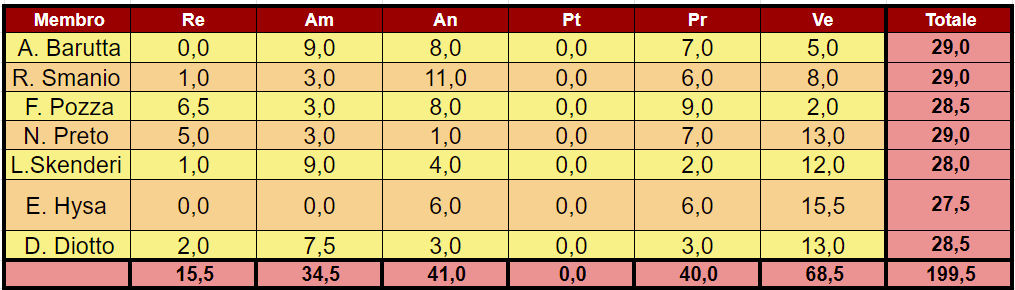
\includegraphics[width=0.9\textwidth]{../Images/riepilogoRTBOreMembro.png}
    \caption{Totale ore impiegate - RTB}
    \label{fig:Tot_oreRTB}
\end{figure}
\begin{figure}[H]
    \centering
    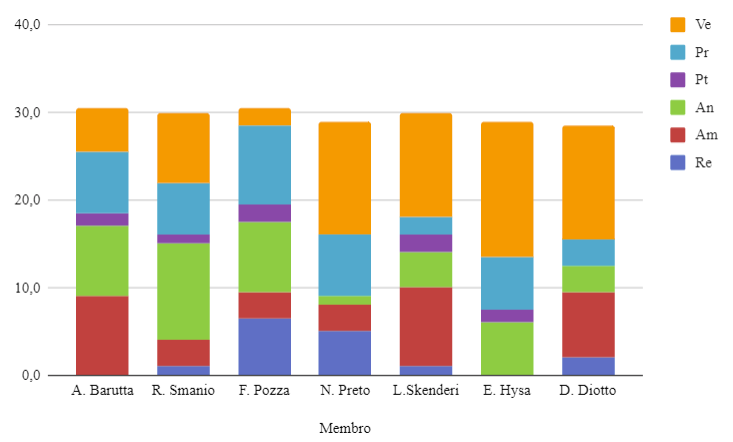
\includegraphics[width=0.8\textwidth]{../Images/graficoOrarioRuoloRTB.png}
    \caption{Istogramma orario ruoli per membro  - RTB}
    \label{fig:GraficoOreRTB}
\end{figure}
\begin{figure}[H]
    \centering
    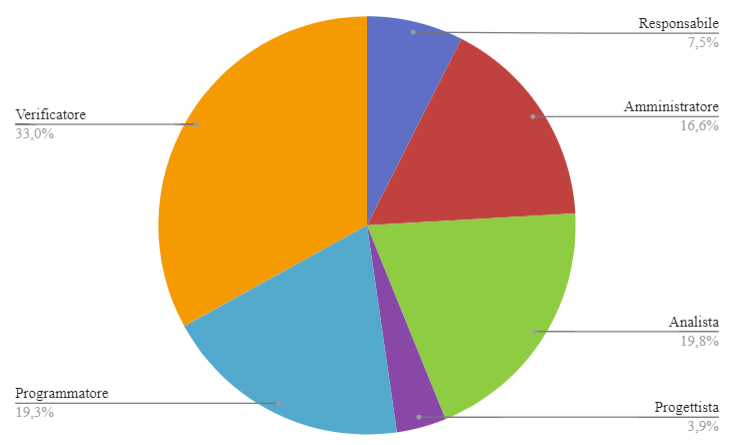
\includegraphics[width=0.8\textwidth]{../Images/distribuzioneOrariaRTBRuoli.png}
    \caption{Distribuzione oraria ruoli  - RTB}
    \label{fig:GraficoDistribuzioneOreRTB}
\end{figure}


\paragraph{Budget}
Il totale dei costi sostenuti dai membri del gruppo, suddivisi per ruolo, è il seguente:
\begin{figure}[H]
    \centering
    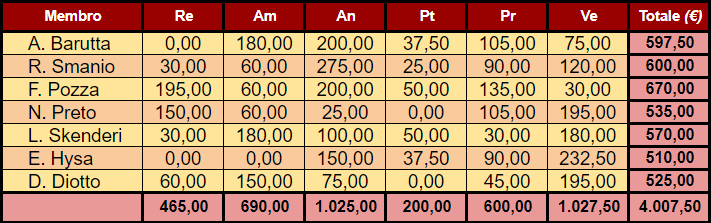
\includegraphics[width=0.9\textwidth]{../Images/RiepilogoPrezziRTB.png}
    \caption{Istogramma orario ruoli per membro  - RTB}
    \label{fig:CostiRTB}
\end{figure}
\begin{figure}[H]
    \centering
    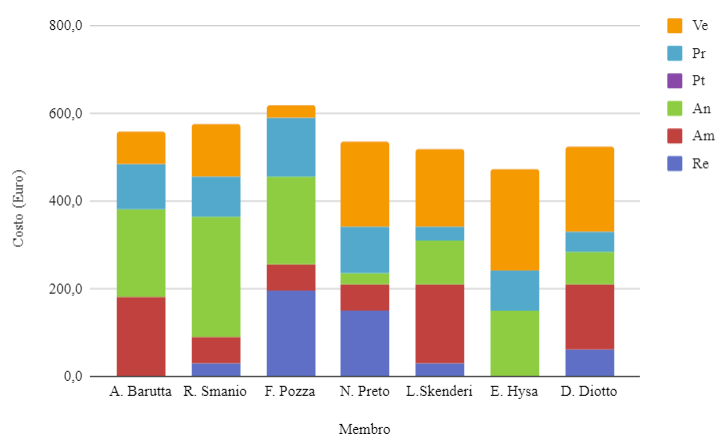
\includegraphics[width=0.8\textwidth]{../Images/graficoCostoRuoloRTB.png}
    \caption{Istogramma costi per membro  - RTB}
    \label{fig:GraficoCostoRTB}
\end{figure}